\section{\system{}: Routing Around Nation-States}
\label{system_design}

\system{} comprises (1)~an overlay network of relays; and (2)~an oracle that
directs clients to the appropriate relays, as shown in Figure~\ref{fig:arch}.
\system{}'s relays are TCP proxy servers that allow clients to access web
content without installing custom software. \system{} uses the measurement
methods described in Section~\ref{avoid_results} to learn paths between
clients, relays, and domains; these results are stored at the oracle, which
uses the data to decide which relay a client in some location should use for
accessing a certain domain while avoiding a certain country.  The oracle
periodically computes paths for many combinations of client AS, destination,
and country.   A client can then query the oracle to determine the appropriate
relay to use to avoid a certain country en route to a particular destination.

After enumerating our design goals for \system{}, we explain each component of
the system in more detail. 

%Once the TCP proxies are established, a client needs
%to learn which proxy to use when accessing a given domain.

%\begin{figure}[t]
%\centering
%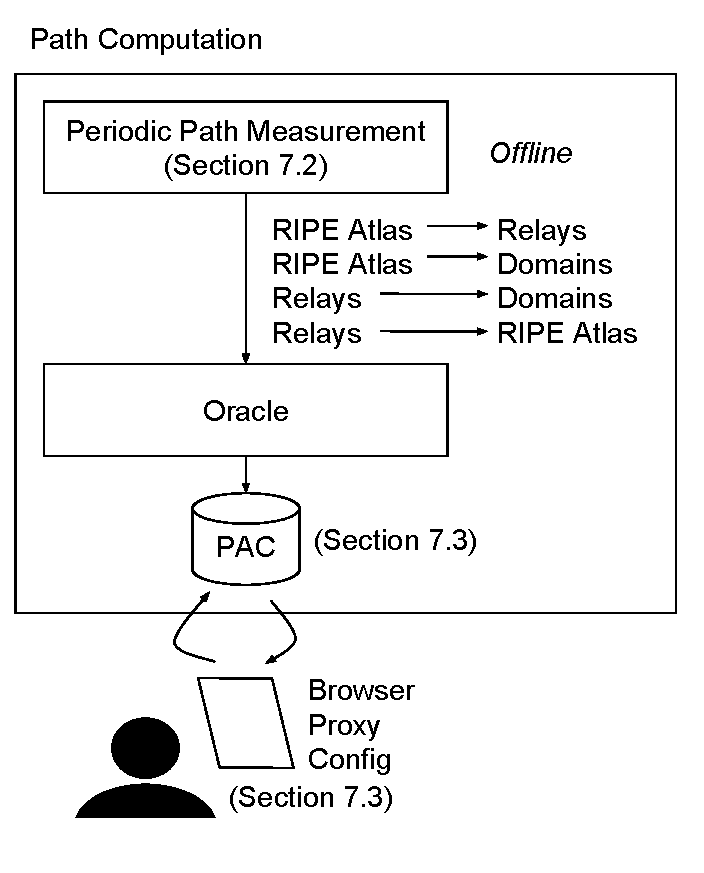
\includegraphics[width=.5\textwidth]{system_overview_updated}
%\caption{\system{} architecture. 1) Paths are computed between clients and relays, 
%relays and domains, relays and clients, and clients and domains.  2) The oracle 
%aggregates all paths.  3)  The oracle generates a PAC file that specifies which 
%domains should be accessed through which relays (based on the measured paths).  
%4) The client configures her browser to use the oracle-generated PAC file.  5) 
%The client's traffic is routed through relays (or direct paths) to access domains, 
%while avoiding a client-specified country.}
%\label{fig:arch}
%\end{figure}

{\bf Design Goals.} Our measurement results motivate 
 the design and implementation of a relay-based avoidance system,
\system{}, with the following design goals.
\label{goals}
\begin{itemize}
\item {\bf Country Avoidance.}  The primary goal of \system{} is to
avoid a given country when accessing web content.  \system{} should
provide clients a way to route around a specified country when
accessing a domain.  This calls for the role of measurement in the
system design and systematizing the measurement methods discussed
earlier in the paper.

\item {\bf Usability.} \system{} should require as little effort as
possible from clients.  Clients should not have to download
or install software, collect any measurements, or understand how the
system works.  This requires a way for clients to automatically and
seamlessly multiplex between relays (proxies) based on different
destinations.  \system{} uses a Proxy Autoconfiguration (PAC) file to support this
function.  PAC files are supported on many types of devices, including mobile 
devices (smartphones, tablets, etc.).  Additionally, this is a mechanism that 
is already being used in systems and tools.  Many Internet users that 
use a VPN have {\it already} used a PAC file; when a user establishes a VPN connection, his 
device's proxy settings are modified to point to a PAC file.  

\item {\bf Scalability.}  This country avoidance system should be able to scale to 
many users.  Therefore, \system{} should be able to handle the addition
 of relays, as well as be cost-effective in terms of resources required. This requires 
clever measurement vantage points, such that each vantage point is representative of 
more than one client.  The PAC file allows \system{} to 
grow with the number of clients and also supports incremental deployment.

\item {\bf Non-goals.}  There are some challenges that \system{} does not
attempt to  solve; in particular, it does not provide anonymity; it routes
around  countries,
but it does not attempt to keep users anonymous in the event that traffic can
be observed.   \system{} also does not address domestic interference or surveillance. For
example, a client in the U.S. cannot use \system{} to avoid network interference 
by the United States. 
\end{itemize}


\subsection{Periodic Path Measurement}

\system{} measures all paths using {\tt 
traceroute}, which is then mapped to the country level using the same methods as 
described in Section~\ref{datasets} and shown in Figure~\ref{fig:analysis_pipeline}.
The paths we measure are the: forward paths from 
the client to each relay; forward paths from each relay to each domain; forward
paths from the client to each domain; and reverse paths from each relay to the 
client. 
%Figure \ref{fig:paths} shows the forward and reverse paths when accessing 
%content using relays; the only path we cannot measure is the reverse path from 
%the domains to the relays because we have no 
%vantage point at or near the domain for running traceroute.
The portion of the reverse path from the domains to the relays is
challenging to measure due to a lack of vantage points in ASes of common
destinations. As discussed in Section \ref{path_sym}, we found that  the
forward and reverse paths are asymmetric at the country level, and therefore
\system{} cannot make any guarantees about which countries are on the path
between  domains and relays even though it has calculated the paths from
relays to domains.   Despite the lack of knowledge about this part of the
reverse path,  we can reason about possible scenarios.  If the client's
traffic is encrypted, then a  on this part of
the reverse path that the client wishes to avoid cannot perform any  traffic correlation
attacks or website
fingerprinting attacks, as the country cannot see who the client is (necessary
for website fingerprinting) and does not have access to more than one part of
the path (necessary for traffic correlation attacks).

\begin{figure}[t!]
    \centering
%    \begin{subfigure}[b]{0.4\textwidth}
        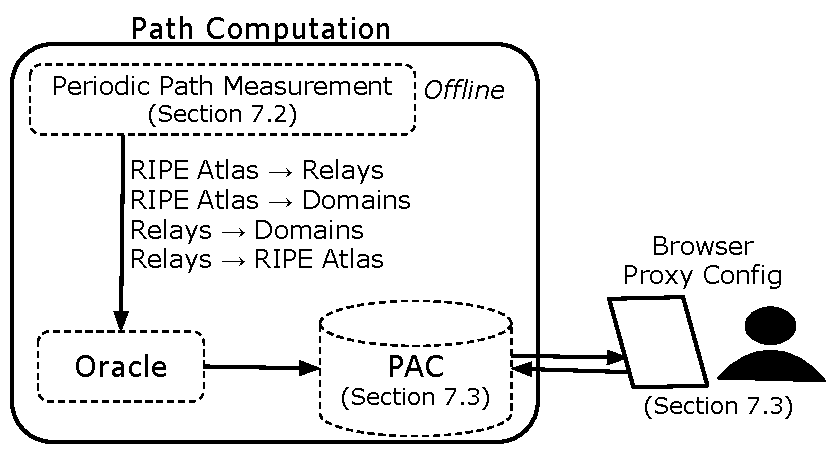
\includegraphics[width=\linewidth]{system_overview_updated-2}
        \caption{\system{} architecture.}
        \label{fig:arch}
%    \end{subfigure}
%    \begin{subfigure}[b]{0.4\textwidth}
%        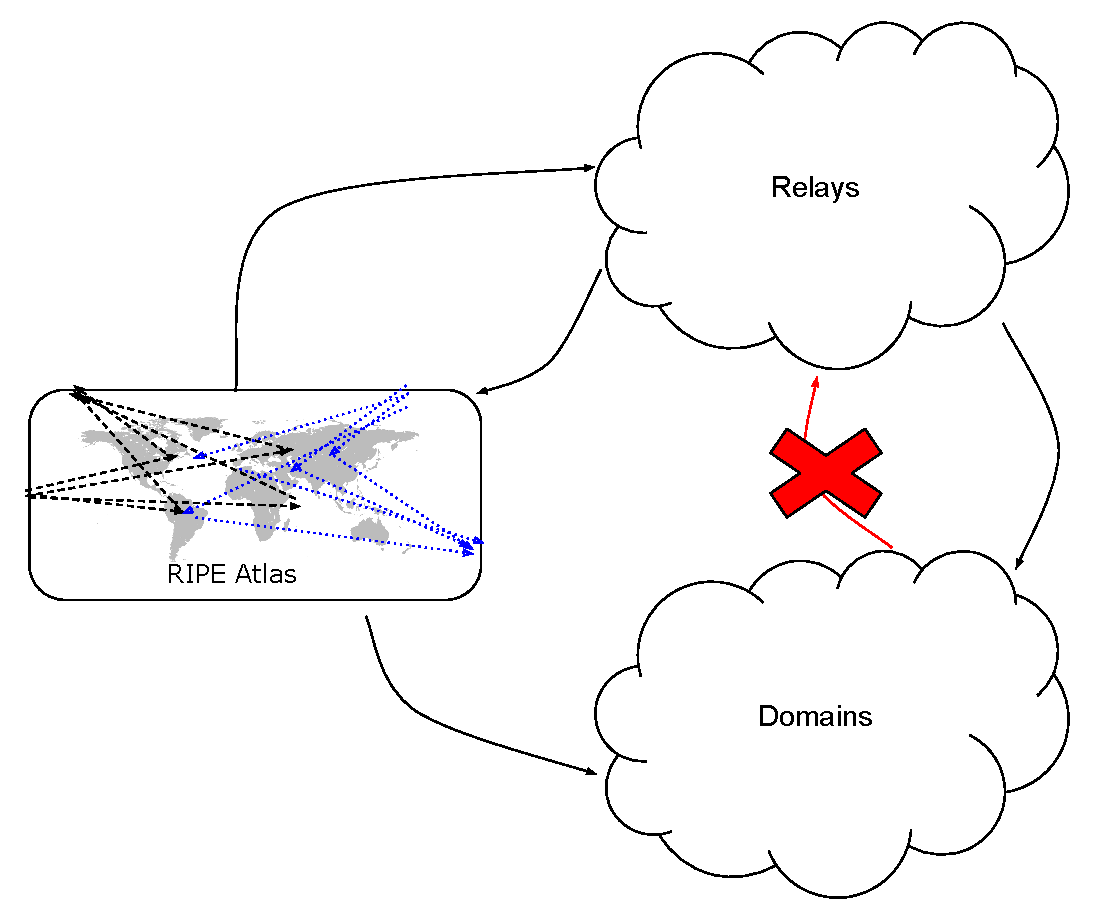
\includegraphics[width=\textwidth,height=7cm]{all_paths}
%        \caption{Paths computed in \system{}.}
%        \label{fig:paths}
%    \end{subfigure}
%    \caption{\system{} architecture, and the path
%      measurements that \system{} periodically computes.}
\end{figure}


\paragraph{Client-to-Relay Paths.} 
To avoid requiring the client to install custom software, \system{}
measures client-to-relay paths from RIPE Atlas probes that serve as 
vantage points for the ASes where \system{} clients might be.  \system{} selects
probes that
are geographically close the client (\eg, in the same 
country). The oracle triggers the probe to run traceroutes
to each relay.  After collecting the responses, the oracle maps 
the IP-level paths to country-level paths and stores the results.

\paragraph{Relay-to-Client Paths.} The \system{} relays perform
traceroutes to the IP addresses of RIPE Atlas probes, which 
represent client ASes.  They then derive country-level paths; the
oracle learns these paths from each relay.  

\paragraph{Relay-to-Server Paths.} Relays perform 
traceroutes to each domain.  As with paths to clients,
relays derive country-level paths and send them to the oracle.

\paragraph{Client to Server Paths.} In case a path from a client to a 
domain does not pass through the country specified to avoid {\it by default}, 
then none of the proxies should be used.  
%If a proxy is used, then it may 
%actually be causing the path to traverse more countries
%(unnecessarily).  
These paths are measured using the RIPE Atlas probes in similar
locations as the clients, and the oracle triggers traceroutes from
each of them to each of the domains.  Corresponding country-level
paths are stored at the oracle.

These paths must be re-computed 
as paths may change.  To our knowledge, there has not been any previous work 
on how often country-level paths change; prior work has explored how often 
AS-level paths change.  We measured the country-level paths from a RIPE Atlas probe to the 
Alexa Top 100 domains once per day for a month to see how stable country-level paths 
are.  Across the measured domains, we found the average time between path changes to 
be about five days.  Therefore, \system{} re-computes the paths every five days to incorporate the 
most recent country-level paths.  

%To measure how often country-level paths change, we 
%computed the paths from relays to domains once every two hours and once every 
%hour.  Fewer than five paths changed every two hours; the 
%results were similar for one-hour increments.  As it takes approximately 30 minutes to 
%compute all paths, \system{} re-computes the paths every one hour to incorporate 
%the most recent country-level paths.

%\begin{figure}[t]
%\centering
%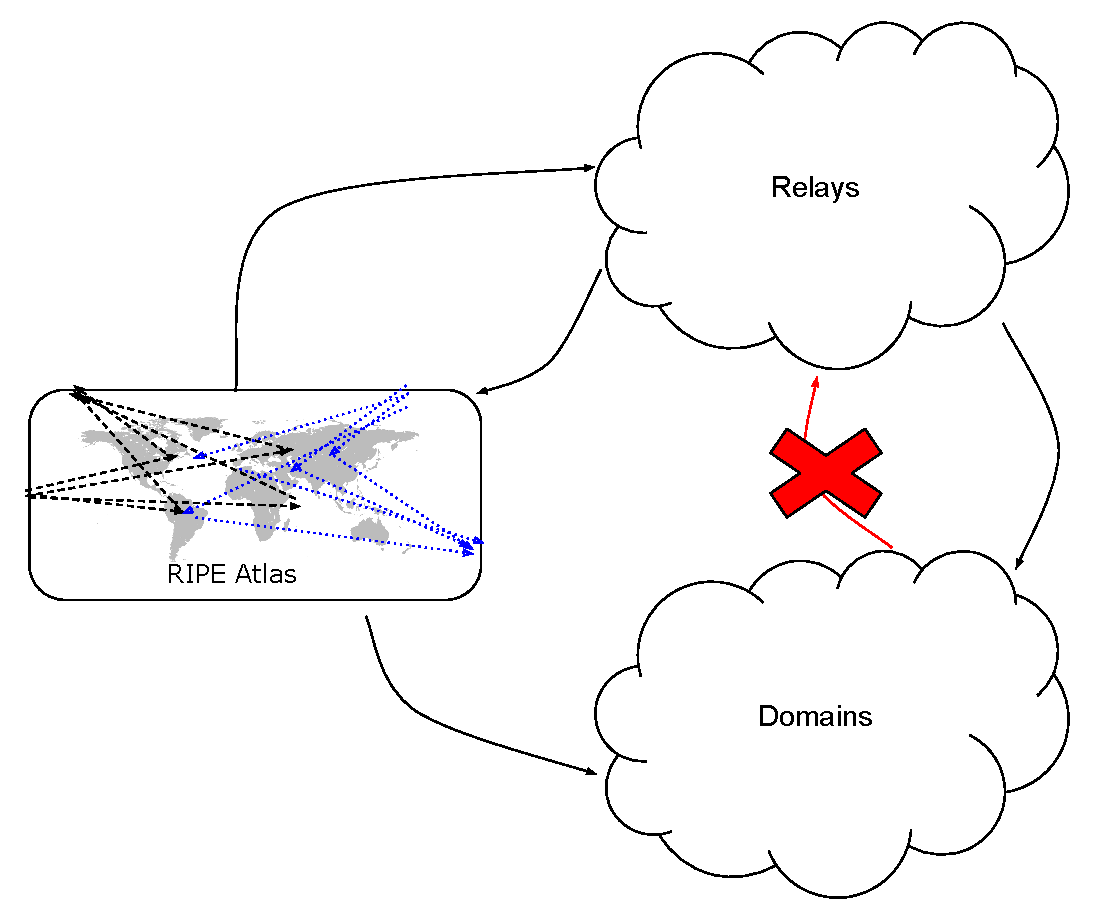
\includegraphics[width=.5\textwidth]{all_paths}
%\caption{The path of a web request through a \system{} relay, to the domain, and back. 
%1) forward path from client to relay; 2) forward path from relay to domain; 3) reverse 
%path from domain to relay; 4) reverse path from relay to client.  \system{} measures 
%all paths except for path 3) due to a lack of vantage points at domain locations.}
%\label{fig:path_components}
%\end{figure}


\subsection{PAC File Generation}
\label{multiplex}
The oracle follows four steps to decide which relay a client should
use to access a specific domain: (1)~If the default path from the
client to the domain does not pass through the specified country, then
do not use any of the relays.  (2)~Otherwise, for all the paths from
the client to the relays, select suitable relays, which are relays where the country 
to avoid is not on the forward or reverse path between the client and 
relay.  (3)~From this set, if there
is a path from a suitable relay to the domain that does not include
the specified country, then use that relay for that domain.  (4)~If
there is no path from the client through any of the relays to the
domain that does not pass through the specified country, then select
the relay that provides the most avoidance (measured by how many other
domains that avoid the specified country).
\begin{figure}[t]
\renewcommand{\lstlistingname}{Configuration}
\lstinputlisting[label={lst:pac}, language=JavaScript, frame=single,
basicstyle=\footnotesize, caption={Example PAC file.}]{example_pac.pac}
\vspace*{-0.25in}
\end{figure}
The oracle applies this decision process to each domain, which results
in a mapping of domains to relays that can be used to avoid the given
country.  To facilitate automatic multiplexing between relays,
\system{} utilizes Proxy Autoconfiguration (PAC) files, which define
how browsers should choose a proxy when fetching a URL.  In the
example PAC file in Configuration~\ref{lst:pac}, proxy 1.2.3.4:3128
should be used when accessing {\tt www.google.com}, but proxy
5.6.7.8:3128 should be used when accessing {\tt www.twitter.com}.  The
oracle uses the mapping of domains to relays to generate a PAC file,
which specifies which domains should be accessed through which proxy.
The PAC file is published online to a URL of the format
$<$client\_country$>$\_$<$country\_to\_avoid$>$\_pac.pac.  The client
uses this URL to specify their proxy configuration.  Paths are
re-computed every five days, so the contents of the PAC file are also
updated every five days.
% The PAC files are published online, which allows a client to simply
% point the proxy configuration settings to the URL that contains the
% PAC file.

\subsection{Scalability and Fault Tolerance}
Adding relays to \system{} is 
straightforward. Additionally, \system{} is resilient to failures of system components.

\paragraph{Adding relays and oracles.} To add a relay, the system
operator must set up a machine as a proxy server, install the relay
software, and update the oracle's list of relays.  From that point
onward, paths will be computed to and from the new relay, and clients
will begin using the new proxy.  Adding an oracle requires installing
the oracle software on a different machine, and specifying the client
locations handled by that oracle (\eg, one oracle handles clients in
North America and Europe, and another handles clients elsewhere).
Both oracles will publish the PAC files to the same server, which
causes no changes for the client.

\paragraph{Failed relays and oracles.} Unresponsive relays are handled
by the PAC file.  The PAC file allows the oracle to specify multiple
proxies in a sequential order, such that if the the first proxy fails,
then the client users the second proxy (and so on).  This feature can
be used to specify all of the relays that have a path to the domain.
%And future work can include relay replicas that can be used in the
%case that a relay crashes.  
Among other mechanisms, we can detect a failed oracle by determining
that its PAC file is older than one hour.  Detecting a failed oracle
could trigger a backup oracle to re-compute the PAC files
periodically.  Because oracles are stateless, failover is
straightforward.  Without backup oracles, clients can still use the
system when the oracle fails.  The clients will simply be using stale
paths, which are likely (but not guaranteed) to be functional, since
country-level paths change infrequently.


